\documentclass[11pt,letterpaper]{article}
\usepackage{style}

%% ------- INICIA DOCUMENTO ------
\begin{document}
\begin{titlepage}
\begin{center}
\begin{LARGE}
INSTITUTO POLITÉCNICO NACIONAL\\
\vspace*{0.15in}
ESCUELA SUPERIOR DE CÓMPUTO\\
\end{LARGE}
\vspace*{1.0in}
\begin{Large}
%% NOMBRE DE LA PRÁCTICA O EXAMEN
\textbf{TÉCNICAS DE CRUZA 1} \\  
\end{Large}
\vspace*{0.2in}
\begin{large}
\textit{Práctica 6}\\
\end{large}
\vspace*{1.0in}
\begin{large}
%% INTEGRANTES	
Dominguez de la Rosa Bryan\\
\vspace*{2.0in}
GRUPO 3CM5\\
\vspace*{0.2in}
Profesor: Morales Güitron Sandra Luz\\
\vspace*{1.5in}
\today
\vspace*{0.3in}
\end{large}
\rule{150mm}{0.1mm}\\

\end{center}
\end{titlepage}

%% --------- COMIENZA EL DESARROLLO DEL DOCUMENTO --------

\section*{Introducción}
Una parte fundamental del funcionamiento de un algoritmo genético es el proceso de selección de candidatos a reproducirse. En los algoritmos genéticos, este proceso suele darse de manera probabilística, es decir, aún los individuos menos aptos tienen una oportunidad de sobrevivir.\\

Los algoritmos de selección proporcional son esquemas en los cuales se eligen individuos de acuerdo a su contribución de aptitud con respecto al total de la población dentro de éstos mecanismos de selección se encuentra el método de \textbf{La ruleta}.\\

La técnica de la ruleta fue propuesta por DeJong y ha sido el método más usado. El algoritmo es simple pero ineficiente, con complejidad $O(n^{2})$.\\

El algoritmo es el siguiente:
\begin{enumerate}
	\item Calcular la suma de valores esperados $T$
	\item Repetir $N$ veces ($N$ es el tamaño de la población):
	\begin{itemize}
		\item Generar un número aleatorio $r$ entre 0.0 y $T$
		\item Ciclar a través de los individuos de la población sumando los valores esperados hasta que la suma sea mayor o igual a $r$
		\item El individuo que haga que esta suma exceda el límite es el seleccionado
	\end{itemize}
\end{enumerate}


\section*{Contenido}
Para la implementación del algoritmo de ruleta, implementé 4 arreglos de bits para controlar las distintas etapas que se realizan en el algoritmo:
\begin{itemize}
	\item Población inicial.
	\item Población de individuos seleccionados por ruleta.
	\item Población después de cruza.
	\item Población después de mutación.
\end{itemize}

En la primer etapa, se llena aleatoriamente el arreglo de población inicial con series de 5 bits. Una vez que se tiene la primer población, se ejecuta el algoritmo de ruleta, de la siguiente forma:

\begin{enumerate}
	\item Se genera un número aleatorio entre 0 y el valor de la aptitud total de la población inicial.
	\item Se genera un ciclo en el que en se acumulará la aptitud total de cada individuo de la población.
	\item El ciclo se detiene cuando la suma acumulada supere el valor aleatorio generado.
	\item El padre seleccionado será el individuo que genere que se sobrepase el valor aleatorio generado. 
\end{enumerate}

\begin{figure}[H]
	\centering
	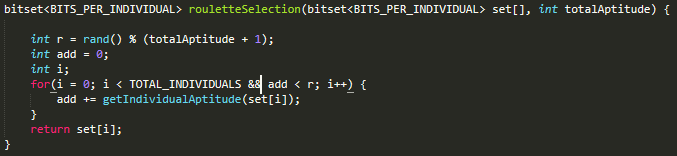
\includegraphics[scale = 1]{images/ruleta}
	\caption{Algoritmo genético de selección de ruleta}
\end{figure}

Una vez teniendo la población de selección de padres, se realiza una cruza de individuos de la siguiente manera:

\begin{enumerate}
	\item Se utilizan 2 individuos de la población de padres.
	\item Se define un punto de cruza estático para todas las generaciones.
	\item Se cruzan los individuos.
	\item Se retorna el individuo resultante.
\end{enumerate}

\begin{figure}[H]
	\centering
	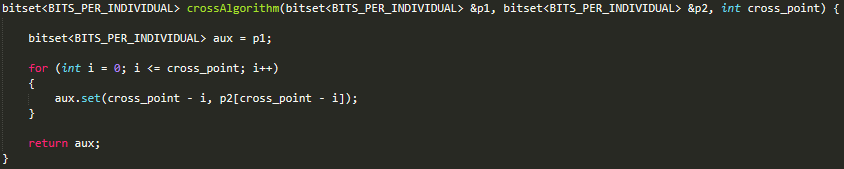
\includegraphics[scale = .8]{images/cruza}
	\caption{Algoritmo de cruza de individuos}
\end{figure}

Al obtener la población de individuos después de la cruza se necesita realizar una mutación. En este caso se generó una mutación del 10\% de la población. Nuestra población total es de 32 elementos, entonces la cantidad de individuos a redondear es 3.2, redondeado como 3.\\

La mutación se realiza de la siguiente forma:
\begin{enumerate}
	\item El algoritmo se realizará 3 veces.
	\item La mutación buscará mejorar al individuo, por lo tanto, se buscará cambiar un bit 0 por un bit 1.
	\item Debido a que se requiere buscar un 0 en el individuo a mutar, y es posible que el individuo no tenga bits 0, se define un número máximo de iteraciones para evitar que el programa se cicle.
	\item Cuando se encuentre un bit 0, se cambia por un bit 1.
\end{enumerate}

\begin{figure}[H]
	\centering
	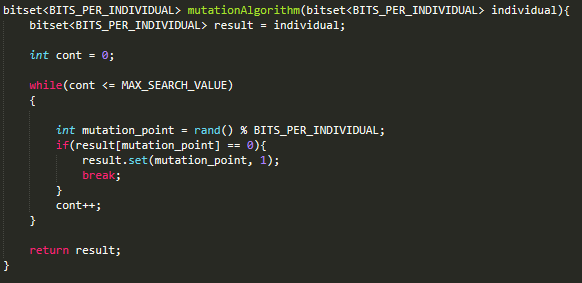
\includegraphics[scale = 1]{images/mutacion}
	\caption{Algoritmo de mutación de individuos}
\end{figure}

Una vez que se tenga la población mutada, se establece ésta como población inicial, para realizar el algoritmo de ruleta en la siguiente generación.\\

Al obtener la población final de una generación, se obtiene la aptitud del individuo de menor valor, la aptitud del individuo de mayor valor y el promedio de aptitud de cada generación.\\

A continuación se muestran 3 ejemplos con 5 generaciones, en los que la línea azul representa la aptitud del mejor individuo de cada generación, la línea roja representa la aptitud del peor individuo de cada generación y la línea blanca representa el promdedio de aptitud de cada generación.
\begin{figure}[H]
	\centering
	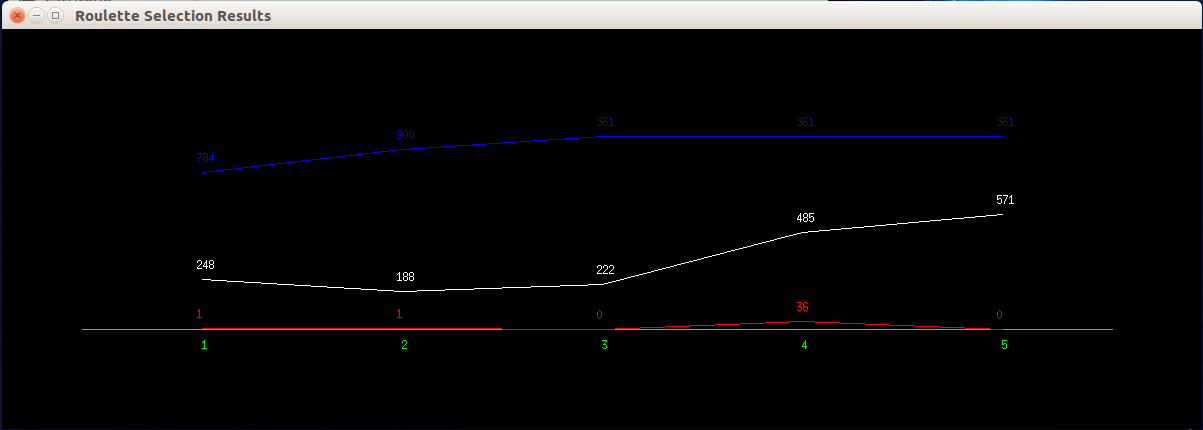
\includegraphics[scale = 0.4]{images/5gen1}
	\caption{Resultado 1 con 5 generaciones}
\end{figure}

\begin{figure}[H]
	\centering
	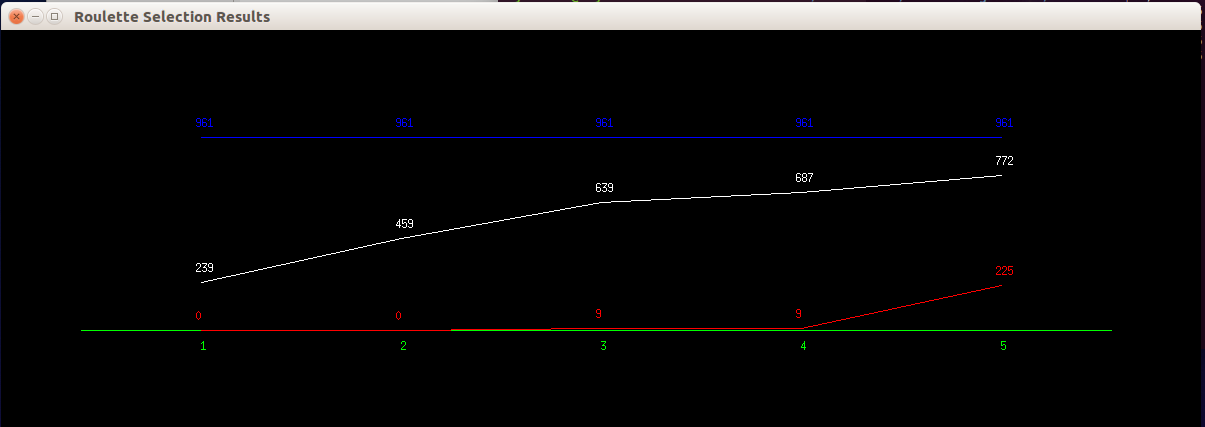
\includegraphics[scale = 0.4]{images/5gen2}
	\caption{Resultado 2 con 5 generaciones}
\end{figure}

\begin{figure}[H]
	\centering
	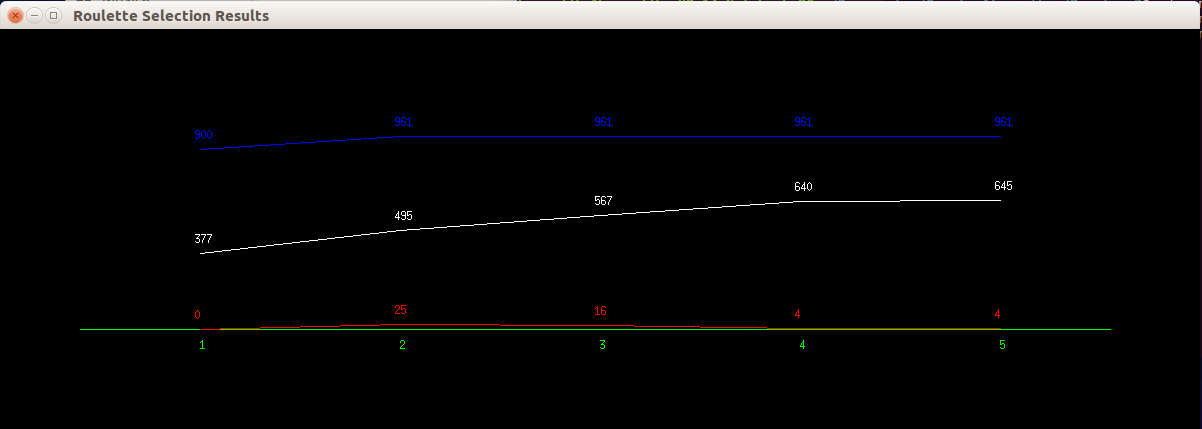
\includegraphics[scale = 0.4]{images/5gen3}
	\caption{Resultado 3 con 5 generaciones}
\end{figure}

A continuación se muestran 3 ejemplos con 10 generaciones:
\begin{figure}[H]
	\centering
	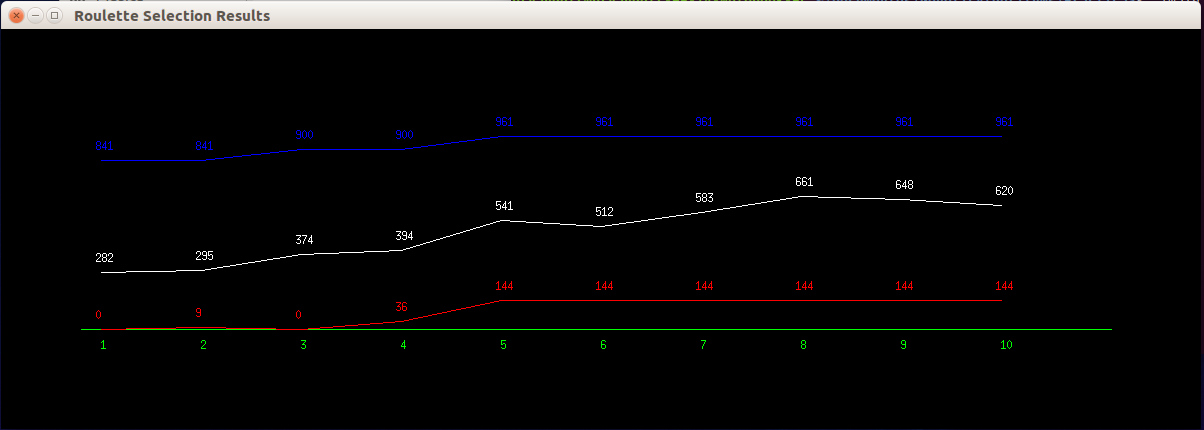
\includegraphics[scale = 0.4]{images/10gen1}
	\caption{Resultado 1 con 10 generaciones}
\end{figure}

\begin{figure}[H]
	\centering
	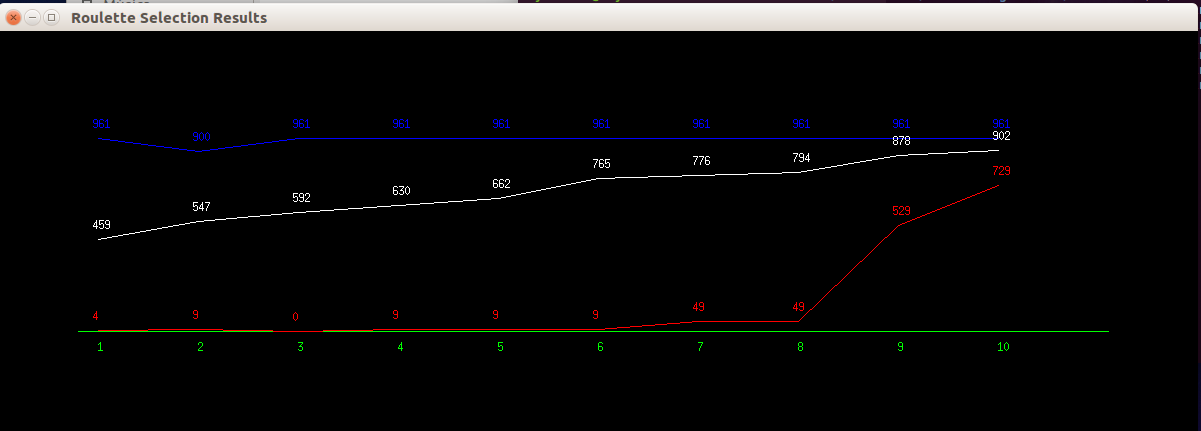
\includegraphics[scale = 0.4]{images/10gen2}
	\caption{Resultado 2 con 10 generaciones}
\end{figure}

\begin{figure}[H]
	\centering
	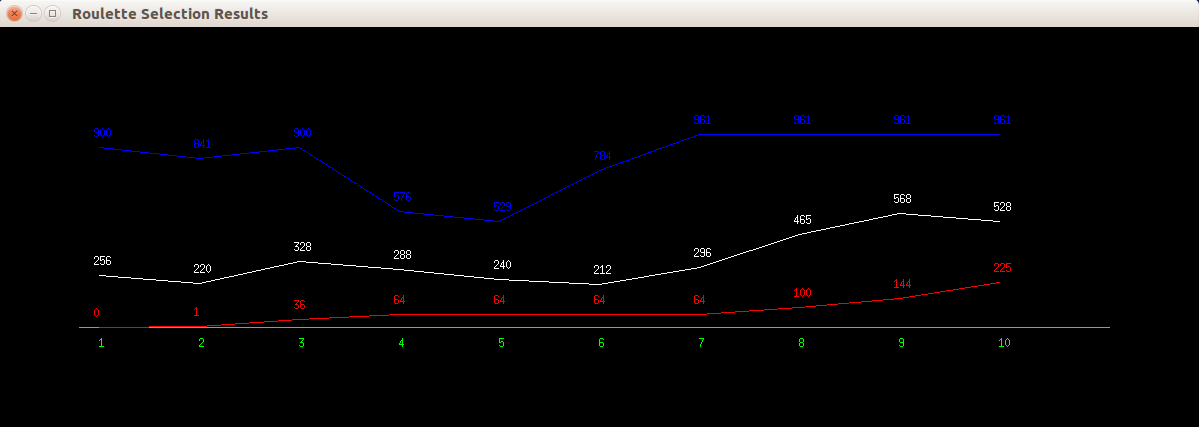
\includegraphics[scale = 0.4]{images/10gen3}
	\caption{Resultado 3 con 10 generaciones}
\end{figure}

A continuación se muestran 3 ejemplos con 15 generaciones:
\begin{figure}[H]
	\centering
	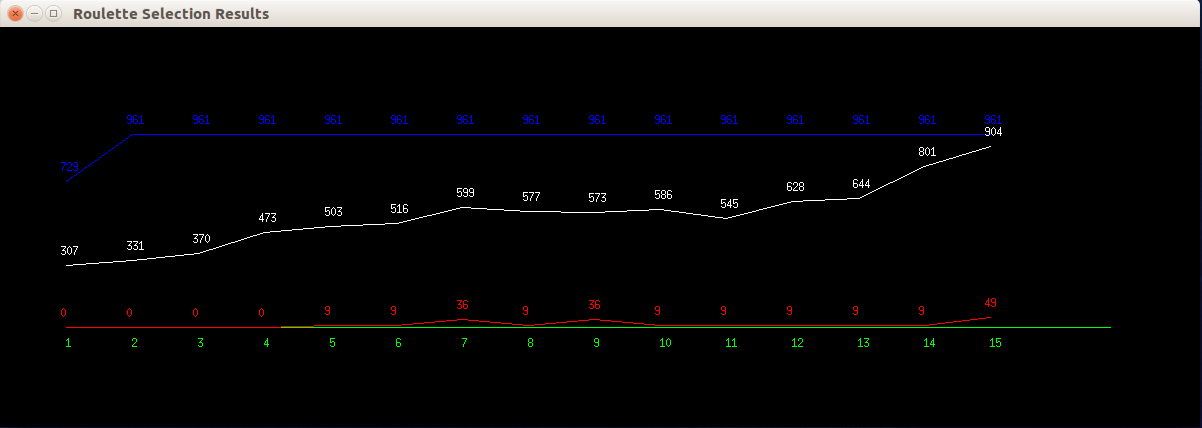
\includegraphics[scale = 0.4]{images/15gen1}
	\caption{Resultado 1 con 15 generaciones}
\end{figure}

\begin{figure}[H]
	\centering
	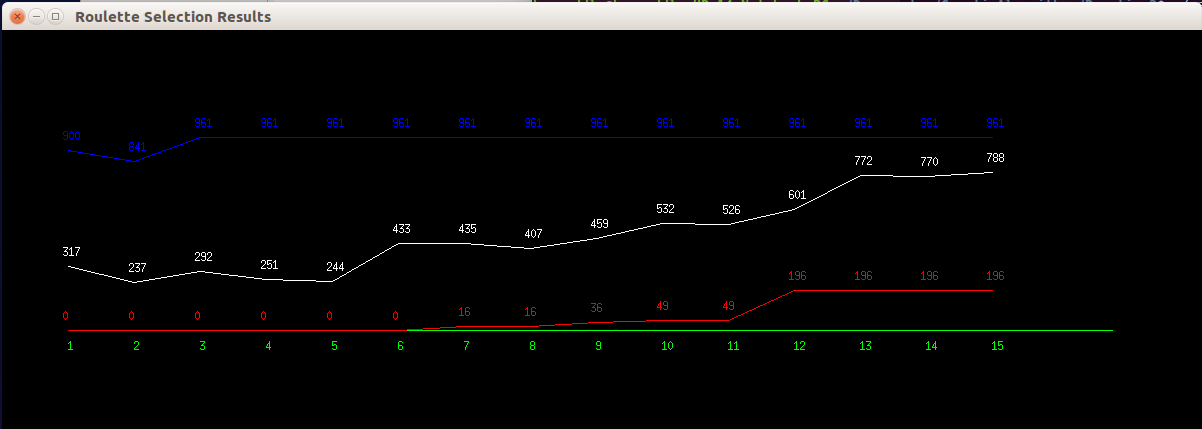
\includegraphics[scale = 0.4]{images/15gen2}
	\caption{Resultado 2 con 15 generaciones}
\end{figure}

\begin{figure}[H]
	\centering
	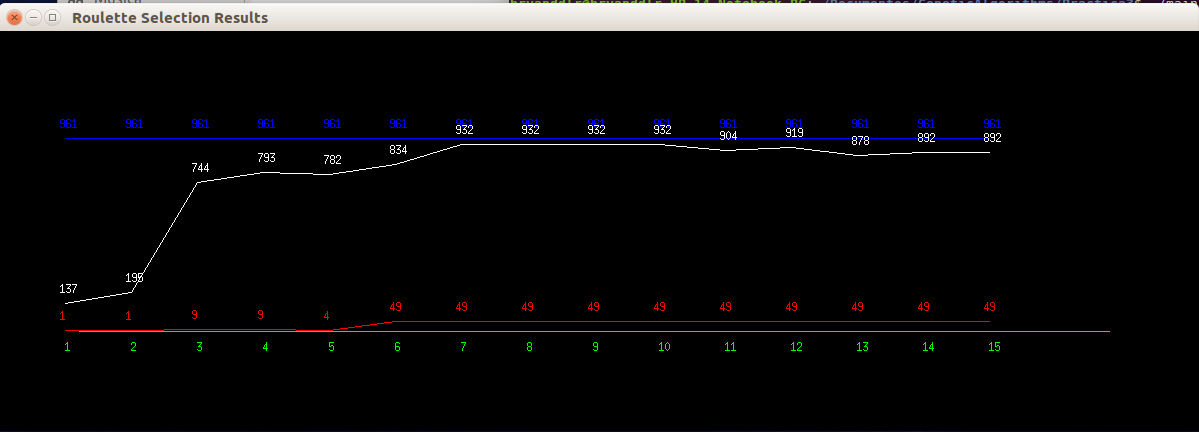
\includegraphics[scale = 0.4]{images/15gen3}
	\caption{Resultado 3 con 15 generaciones}
\end{figure}


\section*{Conclusión}

El fin de un algoritmo genético es simular la evolución de una población de individuos. En esta práctica, utilizamos distintos métodos aleatorios que se presentan en la naturaleza y generan una evolución, tales como la cruza y mutación de individuos, sin olvidar la selección de individuos para siguientes generaciones.\\

El algoritmo genético de selección por ruleta es uno de los más utilizados, sin embargo considero que pueden existir casos en los que la selección de individuos se aplique sobre los individuos de menor aptitud, dado que el número aleatorio de referencia puede ocasionar que se seleccione un individuo con poca aptitud. Aún así, este algoritmo genético permite dar un vistazo de las distintas combinaciones que se presentan en la naturaleza, tanto de flora o fauna, y nos concientiza acerca de que no siempre los individuos más aptos son los que sobreviven, sin embargo, tienen una mayor probabilidad de conseguirlo.


\end{document}


